Hier soll nun ein Verfahren hergeleitet und anschließend mit zwei vereinfachten Verfahren verglichen werden. 

\section{Modellierung}
\label{sec:modellierung}

Für die Erzeugung der Isolationsspektren wird hier das System um den Isolator erweitert und als Zweimassenschwinger (\cref{fig:vkm}) betrachtet.
Wobei der obere Schwinger die aufgehende Struktur ($s$) und der untere Schwinger den Isolator ($i$) samt des steifen Kellergeschosses beschreiben soll.

\begin{figure}[ht]
    \centering
    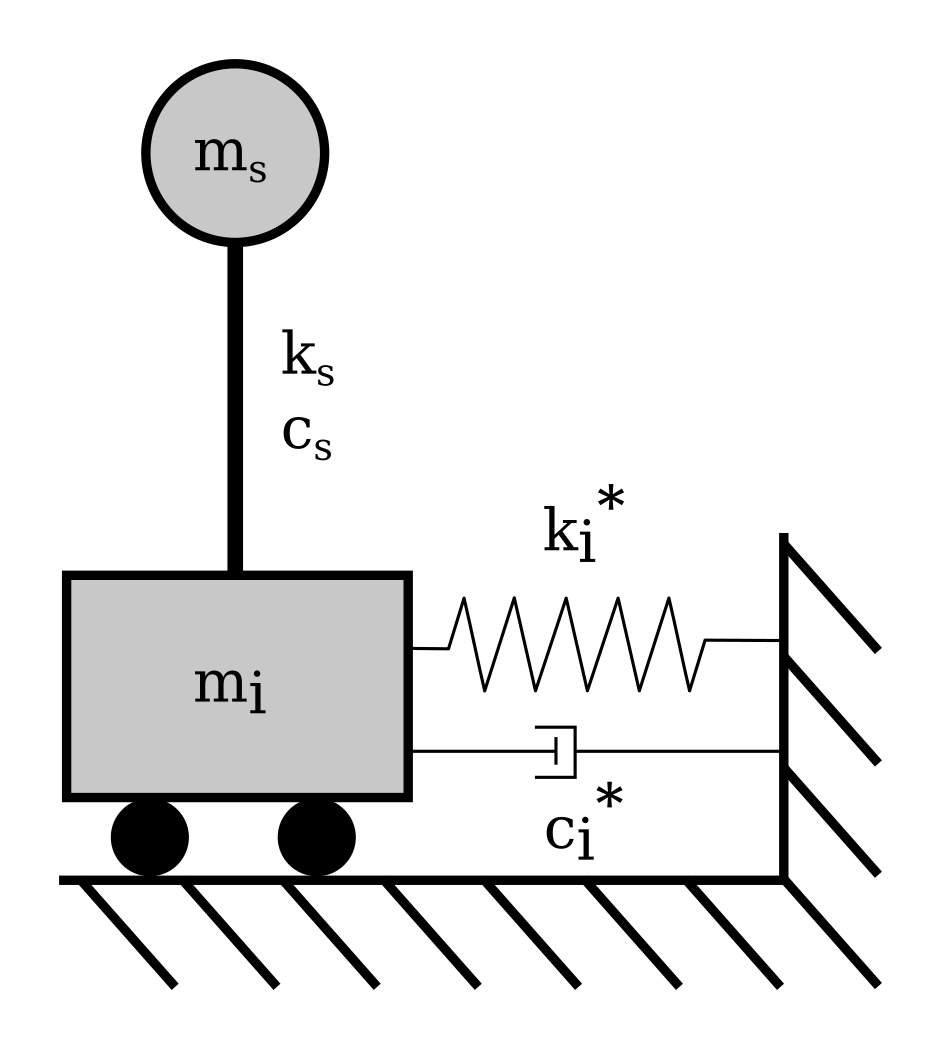
\includegraphics[width=0.5\textwidth]{voigt-kelvin-model.png}
    \caption{Voigt-Kelvin-Modell}
    \label{fig:vkm}
\end{figure}

\subsection{Ansatz über die Übertragsfunktion}
\label{sec:ansatzfunktion}

Der erste untersuchte Ansatz war das Modell in zwei getrennte System zu zerlegen und getrennt zu betrachten.
Die Annahme war, dass der Isolator lediglich als Filter auf das Antwortspektrum wirkt.

\begin{figure}[H]
    \centering
    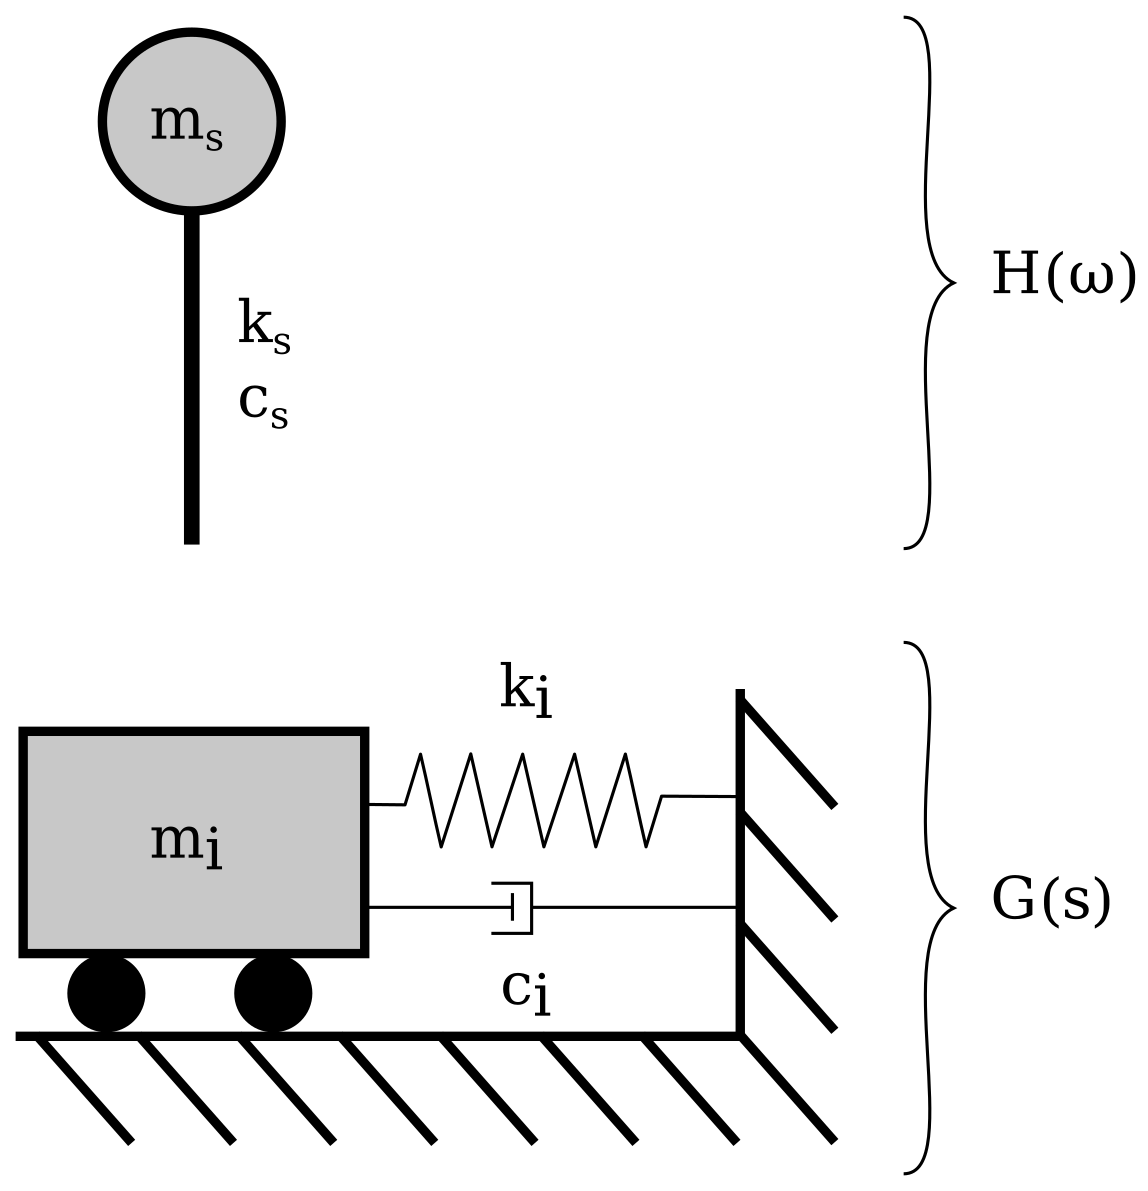
\includegraphics[width=0.7\textwidth]{composition.png}
    \caption{Komposition}
    \label{fig:composition}
\end{figure}

Die Funktion $H(\omega)$ stellt hier das Antwortspektrum dar und $G(s)$ die Übertragungsfunktion des Isolators.
Sie kann mittels der Laplace-Transformation

\begin{equation} \label{laplace}
F(s) = \int_{0}^{\infty} f(t)e^{-st}dt
\end{equation}

aus der Bewegungsgleichung des Isolators \cite{Kramer}

\begin{equation}\label{eq:bewegungsgleichung}
c_i \cdot \dot x(t) + k_i \cdot x(t) = - m_i \cdot \ddot x(t)
\end{equation}

für eine Kraftanregung zu

\begin{equation} \label{laplace2}
G(s)=\frac{X(s)}{F(s)} = \frac{1}{m_i \cdot s^2 + c_i \cdot s + k_i}
\end{equation}

bestimmt (wobei $s = i \omega$) und das isolierte Antwortspektrum ($H(\omega) \cdot |G(s)|$) gewonnen werden da der Betrag der Übertragungsfunktion den Amplitudengang angibt.

Allerdings war dieser Ansatz nicht zielführend, da (wie an den Bewegungsdifferentialgleichungen (\cref{eq:BewegDGL1} und \cref{eq:BewegDGL2}) erkennbar ist) die Systeme gekoppelt sind und nicht getrennt betrachtet werden können.

\subsection{Vereinfachter Ansatz}
\label{sec:ansatzvereinfacht}

Zur Ermittelung der Eigenkreisfrequenzen des Zweimassenschwingers $\omega_{L,1,2}$ werden die Verhältniswerte

\begin{align}
\alpha &= \frac{k_2}{k_1} & \beta  &= \frac{m_2}{m_1} \\
\end{align}

eingeführt. Damit lassen sich die Eigenkreisfrequenzen und Perioden des isolierten Systems bezogen auf die Eigenkreisfrequenz $\omega$ des nicht isolierten Bauwerks wie folgt berechnen \cite{Pocanschi} \cite{Isemann}

\begin{align}
\omega_{L,1}^2 &= \frac{1 + \alpha + \beta - \sqrt{(1 + \alpha + \beta)^2 - 4 \alpha \beta}}{2 \beta} \omega^2\\
\omega_{L,2}^2 &= \frac{1 + \alpha + \beta + \sqrt{(1 + \alpha + \beta)^2 - 4 \alpha \beta}}{2 \beta} \omega^2
\end{align}

\begin{align}
T_{L,1} &= \frac{2 \pi}{\omega_{L,1}} & T_{L,2} &= \frac{2 \pi}{\omega_{L,2}}
\end{align}

Die Komponenten der Eigenvektoren $\vec{\Phi}_{1,2}$ lassen sich über die Beiwerte $\alpha$ und $\beta$ bestimmen.

\begin{align}
r_1 &= \frac{1 + \alpha - \beta + \sqrt{(1 + \alpha + \beta)^2 - 4 \alpha \beta}}{2}\\
r_2 &= \frac{1 + \alpha - \beta - \sqrt{(1 + \alpha + \beta)^2 - 4 \alpha \beta}}{2}
\end{align}

Die Schwingungsformen lauten damit wie folgt und können normiert werden.

\begin{align}
\vec{\Phi}_1 &= \binom{1}{r_1} & \vec{\Phi}_2 &= \binom{1}{r_2}\\
\vec{\Phi}_1 &= \binom{1/r_1}{1} & \vec{\Phi}_2 &= \binom{1/r_1}{1}
\end{align}

Der Beteiligunsfaktor der ersten Schwinungsform wird wie folgt definiert.

\begin{equation}
L_1 = \frac{\vec{\Phi}_1^T M \vec{I}}{\vec{\Phi}_1^T M \vec{\Phi}_1}
\end{equation}

Da die Steifigkeit des Isolators idealerweise deutlich geringer als die der Struktur ist gilt $\alpha \rightarrow 0$, $\vec{I} = \binom{1}{1}$ und $L_2$ wird klein, da die Schwingungsform durch die erste bestimmt wird.
Damit lässt sich die maximale absolute Beschleunigung der Massen der ersten Schwingungsform des Zweimassenschwingers infolge einer Fußpunktanregung bestimmen.

\begin{equation}
\ddot U_{max} = \vec{\Phi}_1 L_1 S_a(T_{L,1}, \xi_{L,1})
\end{equation}

Für die Erzeugung des isolierten Antwortspektrums wird die Steifigkeit der Struktur variiert und die Eigenkreisfrequenz dieser ermittelt.

\begin{equation}
k_{1,i} = \frac{4 \pi^2 m_1}{T_i^2}
\end{equation}

\begin{equation}
\omega = \sqrt{\frac{k_1}{m_1}}
\end{equation}

Da die Antwortspektren im Eurocode auf eine Dämpfung von 5\% normiert sind wird unter der Annahme, dass die Dämpfung des Isolators dominiert das Antwortspektrum abgemindert.

\begin{equation}\label{eta}
\eta = \sqrt{\frac{10}{5 + \xi_2}}
\end{equation}

\subsection{Ansatz über die Transmissibilität}
\label{sec:ansatztrasnm}

Die Beschleunigung aus dem Antwortspektrum wird in eine äquivalente harmonische Beschleunigungsanregung am Fußpunkt umgerechnet.
Anschließend wird über die Bewegungsgleichungen (\cref{eq:2DOF1,eq:2DOF2}) das Verhältnis der Amplituden von Fußpunktanregung zu harmonischer Schwingung an der oberen Masse $m_1$ hergeleitet.
Da die Perioden im Antwortspektrum die Eigenfrequenz des zur Erzeugung verwendeten Einmassenschwingers darstellen, kann eine harmonische Anregung erzeugt werden dessen Erregerfrequenz der Eigenfrequenz des Einmassenschwingers entspricht.
Zur Erzeugung eines isolierten Antwortspektrums soll dann die Steifigkeit $k_1$ variiert werden, sodass die Eigenfrequenz des oberen Systems der Periode des Antwortspektrums entspricht, und die Parameter des Isolators konstant bleiben.
So kann ein Isolationsspektrum erzeugt werden, dass für jede Periode der aufgehenden Struktur eine äquivalente Beschleunigungsantwort angibt.

\subsubsection{Transmissibilität}
\label{sec:transm}

Die Bewegungsdifferentialgleichungen für das in \cref{fig:vkm} dargestellte System lauten:

\begin{align}
\ddot x_1 m_1 &= -(x_1 - x_2) k_1 -(\dot x_1 - \dot x_2) c_1 \label{eq:BewegDGL1}\\
\ddot x_2 m_2 &= (x_1 - x_2) k_1 + (\dot x_1 - \dot x_2) c_1 - (x_2 - x_3) k_2 - (\dot x_2 - \dot x_3) c_2 \label{eq:BewegDGL2}
\end{align}

Ansatz für harmonische Schwingung:

\begin{align*}
x_j &= S_j e^{i \omega t} & \dot x_j &= i \omega S_j e^{i \omega t} & \ddot x_j &= - \omega^2 S_j e^{i \omega t}
\end{align*}

\begin{align}
- \omega^2 S_1 m_1 e^{i \omega t} &= - (S_1 - S_2) e^{i \omega t} k_1 - (S_1 - S_2) i \omega c_1 e^{i \omega t} \label{eq:2DOF1} \\
- \omega^2 S_2 m_2 e^{i \omega t} &= (S_1 - S_2)(k_1 + i \omega c_1) e^{i \omega t} - (S_2 - S_3)(k_2 + i \omega c_2) e^{i \omega t} \label{eq:2DOF2}
\end{align}

\cref{eq:2DOF1} nach $S_2$ umgestellt:

\begin{align*}
\omega^2 S_1 m_1 &= (S_1 - S_2)(k_1 + i \omega c_1) \\
&\Rightarrow X_1 = \frac{\omega^2 m_1}{k_1 + i \omega c_1}\\
S_2 &= S_1 (1 - X_1)
\intertext{$S_2$ in \cref{eq:2DOF2} eingesetzt:}
\omega^2 m_2 S_1 &= - (S_1 - S_1 (1 - X_1)) (k_1 + i \omega c_1) + (S_1 (1 - X_1) - S_3) (k_2 + i \omega c_2)\\
&\Rightarrow X_2 = \frac{\omega^2 m_2}{k_2 + i \omega c_2}\\
S_1 (1 - X_1) X_2 &= S_1 (1-X_1) - S_3 - S_1 X_1 \frac{k_1 + i \omega c_1}{k_2 + i \omega c_2}\\
&\Rightarrow X_{12} = \frac{\omega^2 m_1}{k_2 + i \omega c_2}\\
S_1 (1 - X_1)(X_2 - 1) &= S_3 + S_1 X_{12}\\
S_3 &= S_1 [(1 - X_1)(1 - X_2) - X_{12}]
\end{align*}

Mit den komplexwertigen Transmissionskoeffizienten $X_1$, $X_2$ und $X_{12}$ ergibt sich die Transmissibilität aus dem Betrag des Verhältnisses von $S_1$ zu $S_3$.

\begin{equation}\label{eq:VT2DOF}
VT = \left\lvert \frac{S_1}{S_3} \right\rvert = \left\lvert \frac{1}{[(1 - X_1)(1 - X_2) - X_{12}]} \right\rvert
\end{equation}

Ein Hindernis stellen jedoch noch die Dämpfungsbeiwerte $c_1$ und $c_2$ dar. Die Gleichungen (\ref{eq:BewegDGL1}) und (\ref{eq:BewegDGL2}) können nicht entkoppelt werden und daher kann das, vom Einmassenschwinger gewohnte Lehr'sche Dämpfungsmaß hier nicht angewendet werden.
Ein Ansatz, der hier untersucht werden soll, ist die steifigkeits- und massenproportionale modale Dämpfung. Sie wird auch als Rayleigh-Dämpfung bezeichnet. \cite{Pocanschi}

\subsubsection{Rayleigh-Dämpfung}
\label{sec:rayleigh}

Bei diesem Ansatz soll eine Proportionalität zwischen der Dämpfungsmatrix $C$ und den generalisierten Massen- und Steifigkeitsmatrizen $M^*$ und $K^*$ verwendet werden.

\begin{equation*}
C^* = \alpha M^* + \beta K^*
\end{equation*}

Wobei $\alpha$ und $\beta$ die Beiwerte der Rayleigh-Dämpfung sind.
$\alpha M$ kann als äußere und der Term $\beta K$ als innere Dämpfung verstanden werden.

Die Bestimmungsgleichungen der Beweirte lauten wie folgt.

\begin{align*}
\alpha &= \frac{2 \omega_1^* \omega_2^* (\xi_2 \omega_2^* - \xi_1 \omega_1^*)}{\omega_2^{*2} - \omega_1^{*2}}\\
\beta  &= \frac{2 (\xi_1 \omega_2^* - \xi_2 \omega_1^*)}{\omega_2^{*2} - \omega_1^{*2}}
\end{align*}

Um die Eigenkreisfrequenzen $\omega_1^*$ und $\omega_2^*$ zu erhalten werden zunächst die Eigenkreisfrequenzen am ungedämpften System berechnet und die Eigenvektoren der zugehörigen Eigenformen bestimmt.

Eigenkreisfrequenz des ungedämpften Systems:

\begin{equation*}
\omega_{1,2}^2 = \frac{(k_2 + k_1) m_1 + k_1 m_2 \pm \sqrt{((k_2 + k_1) m_1 + k_1 m_2)^2 - 4 m_2 m_1 k_2 k_1}}{2 m_2 m_1}
\end{equation*}

Eigenvektoren des ungedämpften Systems:

\begin{align*}
\vec{\Phi}_1 &= \binom{\varphi_{11}}{\varphi_{21}} = \binom{1}{\varepsilon_1} & \vec{\Phi}_2 &= \binom{\varphi_{12}}{\varphi_{22}} = \binom{1}{\varepsilon_2}\\
\intertext{mit}
\varepsilon_1 &= \frac{k_2 + k_1 - m_2 \omega_1^2}{k_1} & \varepsilon_2 &= \frac{k_2 + k_1 - m_2 \omega_2^2}{k_1}
\end{align*}

Nach Betragsgröße normierte Eigenvektoren des ungedämpften Systems:

\begin{align*}
\varphi_{11} &= \sqrt{\frac{1}{1 + \varepsilon_1^2}}  &  \varphi_{12} &= \sqrt{\frac{1}{1 + \varepsilon_2^2}}\\
\varphi_{21} &= \varepsilon_1 \varphi_{11}            &  \varphi_{22} &= \varepsilon_2 \varphi_{12}
\end{align*}

Mit Hilfe der Eigenvektoren können die generalisierten Massen und Steifigkeiten ermittelt werden und damit die Eigenkreisfrequenzen.

Generalisierte Massen:

\begin{align*}
m_2^* &= \vec{\Phi}_1^T M \vec{\Phi}_1               &   m_1^* &= \vec{\Phi}_2^T M \vec{\Phi}_2\\
      &= \varphi_{11}^2 m_2 + \varphi_{21}^2 m_1     &         &= \varphi_{12}^2 m_2 + \varphi_{22}^2 m_1
\end{align*}

Generalisierte Steifigkeiten:

\begin{align*}
k_2^* &= \vec{\Phi}_1^T K \vec{\Phi}_1                                                          &   k_1^* &= \vec{\Phi}_2^T K \vec{\Phi}_2\\
      &= \varphi_{11}^2 (k_2 + k_1) - 2 \varphi_{21} \varphi_{11} k_1 + \varphi_{21}^2 k_1      &         &= \varphi_{12}^2 (k_2 + k_1) - 2 \varphi_{22} \varphi_{12} k_1 + \varphi_{22}^2 k_1
\end{align*}

Eigenkreisfrequenzen der zwei Einmassenschwinger:

\begin{align*}
\omega_1^* &= \sqrt{\frac{k_2^*}{m_2^*}}  &  \omega_2^* &= \sqrt{\frac{k_1^*}{m_1^*}}
\end{align*}

Damit ergeben sich die Dämpfungsbeiwerte der Rayleigh-Dämpfung

\begin{align*}
c_1^* &= \alpha m_1^* + \beta k_1^*\\
c_2^* &= \alpha m_2^* + \beta k_2^*
\end{align*}

und die gedämpfte Eigenfrequenz der ersten, durch den Isolator gesteuerten, Eigenform  

\begin{align*}
\omega_{1d} &= \omega_1^* \sqrt{1 - \xi_2^2}\\
T_1         &= \frac{2 \pi}{\omega_{1d}} 
\end{align*}

Die Transmissibilität kann nun mit den Dämpfungsbeiwerten der Rayleigh-Dämpfung bestimmt werden.

\begin{equation}
VT(m_2^*, k_2^*, c_2^*, m_1^*, k_1^*, c_1^*)
\end{equation}

\subsubsection{Erzeugung des isolierten Antwortspektrums}
\label{sec:transmAWS}

Das isolierte Antwortspektrum kann nun aus dem elastischen Antwortspektrum erlangt werden.
Für jede Periode $T_i$ wird die Steifigkeit der aufgehenden Struktur berechnet wobei die restlichen Parameter konstant bleiben.

\begin{equation}
k_{1,i} = m_1 (\frac{2 \pi}{T_i})^2
\end{equation}
  
Damit können die Transmissibilität $VT$, die gedämpfte erste Eigenkreisfrequenz $\omega_{1d}$

\begin{align}
\omega_{1d} &= \omega_1^* \sqrt{1 - \xi_2^2} \\
T_1 &= \frac{2 \pi}{\omega_{1d}}
\end{align}

und die zugehörige äquivalente Amplitude der Beschleunigung der Fußpunktanregung

\begin{equation}
S_{a,x_3} = Se(T_1) / 10.05
\end{equation}

ermittelt werden. Die Ordinate des isolierten Antwortspektrums beträgt dann

\begin{equation}
S_{a,isoliert} = S_{a,x_3} \cdot VT
\end{equation}
  
\pagebreak

\section{Vergleich der Ansätze am Beispiel}
\label{sec:vergleich}

Die Ansätze sollen anhand eines konkreten Beispiels verglichen werden. Hierzu werden die Werte aus \cite{Isemann} Kapitel 11.2.3 verwendet.
Die Parameter des Systems lauten:

\makebox[1cm]{$D$}    = 0.35 m \par
\makebox[1cm]{$\mu$}  = 0.04\par
\makebox[1cm]{$m_1$}  = 2486.7 t\par
\makebox[1cm]{$m_2$}  = 1619.5 t\par
\makebox[1cm]{$R$}    = 2.5 m\par

Es soll ein Antwortspektrum mit folgenden Eckperioden und Bodenbeschleunigung verwendet werden.

\makebox[1cm]{$T_B$}  = 0.4 s\par
\makebox[1cm]{$T_C$}  = 1.6 s\par
\makebox[1cm]{$T_D$}  = 2.0 s\par
\makebox[1cm]{$a_g$}  = 3.924 m/s\textsuperscript{2}\par

\begin{figure}[H]
    \centering
    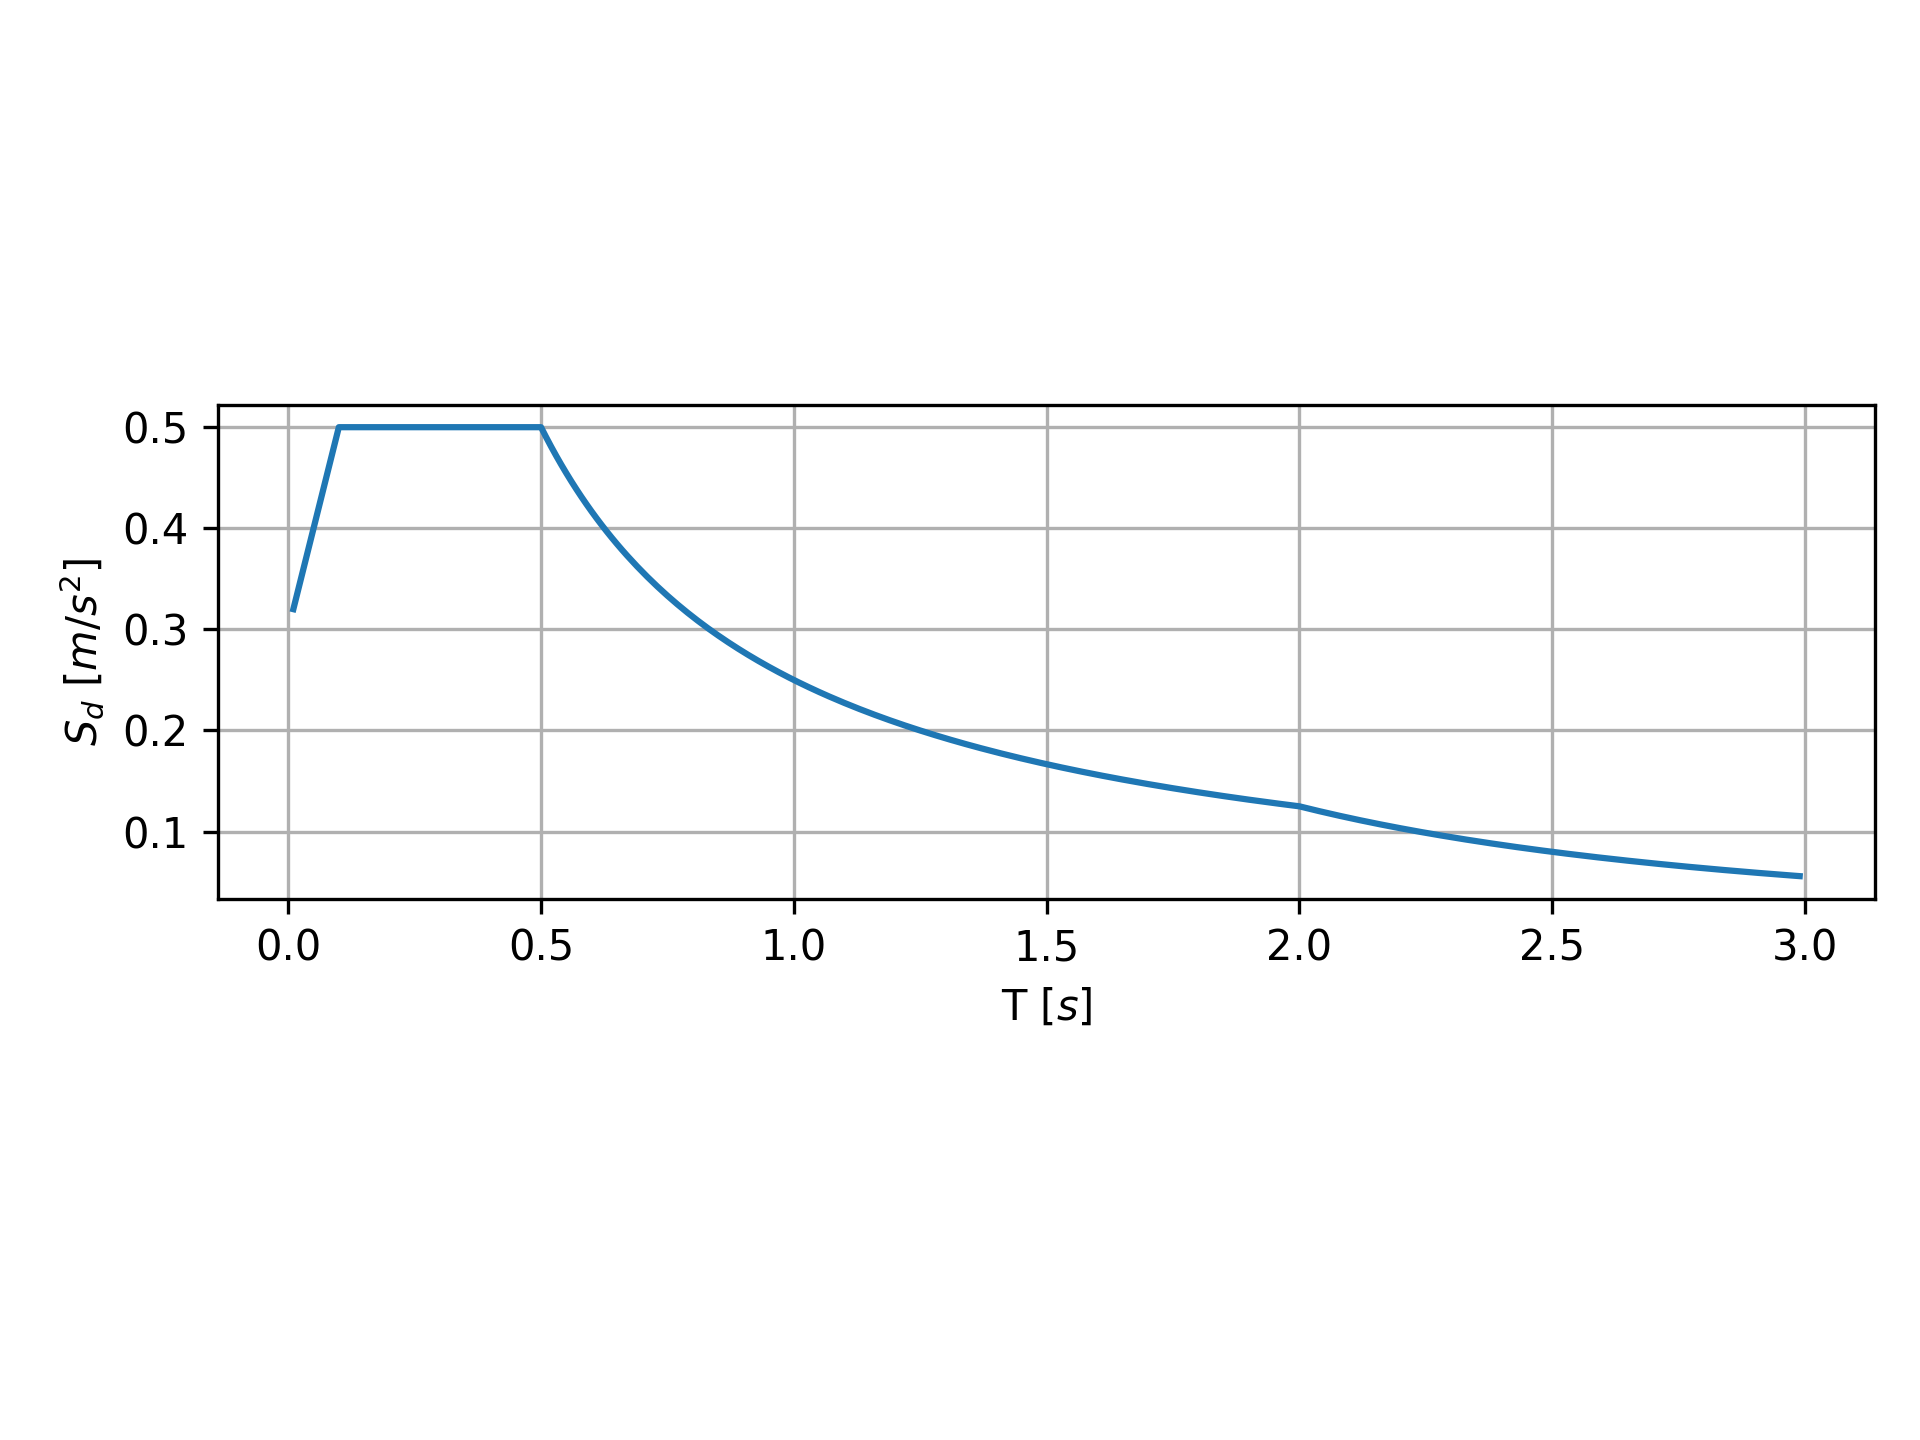
\includegraphics[width=0.9\textwidth]{AWS_beispiel.png}
    \caption{Antwortspektrum}
\end{figure}

Die Steifigkeit $k_2$ ergibt sich aus der effektiven Steifigkeit des Isolators nach \cref{keff}

\begin{equation*}
k_2 = k_{eff} = \frac{G}{R} + \mu \frac{G}{D} = \frac{41062 kN}{2.5 m} + 0.04 \cdot \frac{41062 kN}{0.35 m} = 21117 kN/m
\end{equation*}

Die Dämpfung $\xi_1$ wird mit 5\% angenommen und die effektive Dämpfung des Isolators $\xi_2$ nach \cref{xieff} bestimmt.

\begin{equation*}
\xi_2 = \xi_{eff} = \frac{2}{\pi} \frac{\mu R}{(D + \mu R)} = \frac{2}{\pi} \frac{0.04 \cdot 2.5 m}{(0.35 m + 0.04 \cdot 2.5 m)} \approx 0.14147
\end{equation*}

Hier sollen zunächst die Ergebnisse für eine Periode der aufgehenden Struktur von $T = 1 s$ betrachtet werden. Daraus ergibt sich eine Steifigkeit $k_1$ von

\begin{equation*}
k_1 = m_1 (\frac{2 \pi}{T})^2 = 2486.7 t \cdot (\frac{2 \pi}{1 s})^2 = 98170 kN/m
\end{equation*}

\subsection{Betrachtung als effektiver Einmassenschwinger}

Wie in \cref{sec:schwierigkeitenvordimensionierung} erwähnt kann das System unter der Annahme, dass der Isolator die Eigenform dominiert (\cref{Verteilung}) auch als verienfachter Einmassenschwinger modelliert werden.

Die Eigenperiode beträgt dann

\begin{equation*}
\omega = \sqrt{\frac{k_2}{m_1 + m_2}} = \sqrt{\frac{21117 kN/m}{4106.2 t}} \approx 2.267 \frac{1}{s}
\end{equation*}

\begin{equation*}
T = \frac{2 \pi}{\omega} = \frac{2 \pi}{2.267 \frac{1}{s}} \approx 2.77 s
\end{equation*}

Für eine Periode von $T = 2.77 s$ im Bereich $T_D \leq T$ und, unter der Annahme, dass auch die Dämpfung des Isolators dominiert, $\eta=\sqrt{10/(5+14.147)} \approx 0.723$ beträgt die Spektralbeschleunigung

\begin{align*}
S_a(T) &= a_g \eta 2.5 \frac{T_C T_D}{T^2}\\
       &= 3.924 m/s^2 \cdot 0.723 \cdot 2.5 \cdot \frac{1.6 s \cdot 2.0 s}{(2.77 s)^2}\\
       &= \underline{\underline{2.958 m/s^2}}
\end{align*}

\subsection{Vereinfachtes Verfahren}

Im ersten Schritt wird die Eigenkreisfrequenz des nicht isolierten Bauwerks $\omega$ und die Verhältniswerte $\alpha$ und $\beta$ ermittelt.

\begin{align*}
\omega &= \sqrt{\frac{k_1}{m_1}} = \sqrt{\frac{98170 kN/m}{2486.7 t}} = 6.2832 \frac{1}{s}\\
\end{align*}

\begin{align*}
\alpha &= \frac{k_2}{k_1} = \frac{21117 kN/m}{98170 kN/m} = 0.2151 & \beta  &= \frac{m_2}{m_1} = \frac{1619.5 t}{2486.7 t} = 0.65\\
\end{align*}

Damit lassen sich die Eigenkreisfrequenzen und Perioden des isolierten Systems bestimmen.

\begin{align*}
\omega_{L,1}^2 &= \frac{1 + \alpha + \beta - \sqrt{(1 + \alpha + \beta)^2 - 4 \alpha \beta}}{2 \beta} \omega^2\\
               &= \frac{1 + 0.215 + 0.65 - \sqrt{(1 + 0.215 + 0.65)^2 - 4 \cdot 0.215 \cdot 0.65}}{2 \cdot 0.65} \cdot (6.2832 \frac{1}{s})^2\\
               &= 4.7504 \Rightarrow  \omega_{L,1} = 2.18 \frac{1}{s}\\
\end{align*}

\begin{align*}
T_{L,1} &= \frac{2 \pi}{\omega_{L,1}} = \frac{2 \pi}{2.18 \frac{1}{s}} = 2.882 s
\end{align*}

Für die Periode von $T = 2.77 s$ im Bereich $T_D \leq T$ und der Dämpfung des Isolators mit $\eta=\sqrt{10/(5+14.147)} \approx 0.723$ beträgt die Spektralbeschleunigung

\begin{align*}
S_a(T) &= a_g \eta 2.5 \frac{T_C T_D}{T^2}\\
       &= 3.924 m/s^2 \cdot 0.723 \cdot 2.5 \cdot \frac{1.6 s \cdot 2.0 s}{(2.882 s)^2}\\
       &= 2.733 m/s^2
\end{align*}

Um dann die maximale Beschleunigung zu erhalten wird noch der erste Eigenvektor und Beteiligungsfaktor berücksichtigt.

\begin{align*}
r_1 &= \frac{1 + \alpha - \beta + \sqrt{(1 + \alpha + \beta)^2 - 4 \alpha \beta}}{2} \\
    &= \frac{1 + 0.215 - 0.65 + \sqrt{(1 + 0.215 + 0.65)^2 - 4 \cdot 0.215 \cdot 0.65}}{2}\\
    &= 1.137
\end{align*}

\begin{align*}
\vec{\Phi}_1 &= \binom{1/r_1}{1} = \binom{1/1.137}{1} = \binom{0.8795}{1}
\end{align*}

\begin{equation*}
L_1 = \frac{\vec{\Phi}_1^T M \vec{I}}{\vec{\Phi}_1^T M \vec{\Phi}_1} = \frac{
\begin{pmatrix}
  0.8795 & 1
\end{pmatrix}
\begin{bmatrix}
  1619.5 t & 0 t\\
  0 t & 2486.7 t
\end{bmatrix}
\begin{pmatrix}
  1\\
  1
\end{pmatrix}
}{
\begin{pmatrix}
  0.8795 & 1
\end{pmatrix}
\begin{bmatrix}
  1619.5 t & 0 t\\
  0 t & 2486.7 t
\end{bmatrix}
\begin{pmatrix}
  0.8795 \\
  1
\end{pmatrix}}
= 1.0458
\end{equation*}

\begin{equation*}
\ddot U_{max} = \vec{\Phi}_1 L_1 S_a(T_{L,1}, \xi_{L,1}) = 1.0 \cdot 1.0458 \cdot 2.733 m/s^2 = \underline{\underline{2.858 m/s^2}}
\end{equation*}

\subsection{Verfahren der Transmissibilität}

Zunächst werden die Dämpfungsbeiwerte mit dem Ansatz der Rayleigh-Dämpfung ermittelt. Dafür werden die Eigenkreisfrequenzen des ungedämpften Systems benötigt.

\begin{align*}
\omega_{1,2}^2 &= \frac{(k_2 + k_1) m_1 + k_1 m_2 \pm \sqrt{((k_2 + k_1) m_1 + k_1 m_2)^2 - 4 m_2 m_1 k_2 k_1}}{2 m_2 m_1}\\
               \intertext{mit $(k_2 + k_1) m_1 + k_1 m_2 = (21117  + 98170 ) \cdot 2486.7  + 98170  \cdot 1619.5 = 455568212.9 $ \newline und $4 m_2 m_1 k_2 k_1 = 4 \cdot 1619.5  \cdot 2486.7  \cdot 21117  \cdot 98170 = 3.3370719 \cdot 10^{14}$}
               &= \frac{ 455568212.9 \pm \sqrt{((21117  + 98170 ) \cdot 2486.7  + 98170  \cdot 1619.5 )^2 - 3.33.. \cdot 10^{14}}}{2 \cdot 1619.5  \cdot 2486.7 }\\
               &\Rightarrow \omega_1 \approx 2.179 \frac{1}{s}\\
               &\Rightarrow \omega_2 \approx 10.410 \frac{1}{s}
\end{align*}

Damit können die normierten Komponenten der Eigenvektoren bestimmt werden.

\begin{align*}
\varepsilon_1 &= \frac{k_2 + k_1 - m_2 \omega_1^2}{k_1} \\
              &= \frac{21117 kN/m + 98170 kN/m - 1619.5 t \cdot (2.179 \frac{1}{s})^2}{98170 kN/m}\\
              &= 1.136
\end{align*}
\begin{align*}
\varepsilon_2 &= \frac{k_2 + k_1 - m_2 \omega_2^2}{k_1} \\
              &= \frac{21117 kN/m + 98170 kN/m - 1619.5 t \cdot (10.410 \frac{1}{s})^2}{98170 kN/m}\\
              &= -0.572
\end{align*}

\begin{align*}
\varphi_{11} &= \sqrt{\frac{1}{1 + \varepsilon_1^2}} = \sqrt{\frac{1}{1 + 1.136^2}} \approx 0.660\\
\varphi_{21} &= \varepsilon_1 \varphi_{11} = 1.136 \cdot 0.660 \approx 0.750\\
\varphi_{12} &= \sqrt{\frac{1}{1 + \varepsilon_2^2}} = \sqrt{\frac{1}{1 + (-0.572)^2}} \approx 0.867\\
\varphi_{22} &= \varepsilon_2 \varphi_{12} = -0.572 \cdot 0.867 \approx -0.497
\end{align*}

Die generalisierten Massen und Steifigkeiten sind dann

\begin{align*}
m_2^* &= \varphi_{11}^2 m_2 + \varphi_{21}^2 m_1 = 0.660^2 cdot 1619.5 t + 0.750^2 \cdot 2486.7 t\\
      &= 2108.3 t\\[2em]
m_1^* &= \varphi_{12}^2 m_2 + \varphi_{22}^2 m_1 = 0.867^2 \cdot 1619.5 t + -0.497^2 \cdot 2486.7 t\\
      &= 1833.8 t\\[2em]
k_2^* &= \varphi_{11}^2 (k_2 + k_1) - 2 \varphi_{21} \varphi_{11} k_1 + \varphi_{21}^2 k_1\\
      &= 0.660^2 \cdot (21117 kN/m +  98170 kN/m) - 2 \cdot 0.750 \cdot 0.660 \cdot 98170 kN/m\\
      &\phantom{{}=1} + 0.750^2 \cdot  98170 kN/m\\
      &= 10013.4 kN/m\\[2em]
k_1^* &= \varphi_{12}^2 (k_2 + k_1) - 2 \varphi_{22} \varphi_{12} k_1 + \varphi_{22}^2 k_1\\
      &= 0.867^2 \cdot (21117 kN/m +  98170 kN/m) - 2 \cdot -0.497 \cdot 0.867 \cdot 98170 kN/m\\
      &\phantom{{}=1} + -0.497^2 \cdot 98170 kN/m\\
      &= 198759.0 kN/m
\end{align*}

und die Eigenkreisfrequenzen der zwei Einmassenschwinger

\begin{align*}
\omega_1^* &= \sqrt{\frac{k_2^*}{m_2^*}} = \sqrt{\frac{10013.4 kN/m}{2108.3 t}}\\
           &= 2.179 \frac{1}{s}
\end{align*}
\begin{align*}
\omega_2^* &= \sqrt{\frac{k_1^*}{m_1^*}} = \sqrt{\frac{198759.0 kN/m}{1833.8 t}}\\
           &= 10.410 \frac{1}{s}
\end{align*}

Damit ergeben sich die Dämpfungsbeiwerte der Rayleigh-Dämpfung

\begin{align*}
\alpha &= \frac{2 \omega_1^* \omega_2^* (\xi_2 \omega_2^* - \xi_1 \omega_1^*)}{\omega_2^{*2} - \omega_1^{*2}}\\
       &= \frac{2 \cdot 2.179 \frac{1}{s} \cdot 10.410 \frac{1}{s} \cdot (0.14147 \cdot 10.410 \frac{1}{s} - 0.05 \cdot 2.179 \frac{1}{s})}{(10.410 \frac{1}{s})^2 - (2.179 \frac{1}{s})^2}\\
       &\approx 0.597\\[2em]
\beta  &= \frac{2 (\xi_1 \omega_2^* - \xi_2 \omega_1^*)}{\omega_2^{*2} - \omega_1^{*2}}\\
       &= \frac{2 \cdot (0.05 \cdot 10.410 \frac{1}{s} - 0.14147 \cdot 2.179 \frac{1}{s})}{(10.410 \frac{1}{s})^2 - (2.179 \frac{1}{s})^2}\\
       &\approx 0.004
\end{align*}

\begin{align*}
c_1^* &= \alpha m_1^* + \beta k_1^* = 0.597 \cdot 1833.8 t + 0.004 \cdot 198759.0 kN/m\\
      &\approx 1909.1\\
c_2^* &= \alpha m_2^* + \beta k_2^* = 0.597 \cdot 1833.8 t + 0.004 \cdot 10013.4 kN/m\\
      &\approx 1300.0
\end{align*}

und die gedämpfte Eigenfrequenz der ersten, durch den Isolator gesteuerten, Eigenform  

\begin{align*}
\omega_{1d} &= \omega_1^* \sqrt{1 - \xi_2^2} = 2.179 \frac{1}{s} \cdot \sqrt{1 - 0.14147^2}\\
            &\approx 2.157 \frac{1}{s}\\
T_1         &= \frac{2 \pi}{\omega_{1d}} = \frac{2 \pi}{2.157 \frac{1}{s}}\\
            &\approx 2.912 s
\end{align*}

Mit der Periode lässt sich bereits $S_a$ aus dem Antwortspektrum (mit $\eta=\sqrt{10/(5+14.147)} \approx 0.723$) ermitteln.

\begin{align*}
S_a(T) &= a_g \eta 2.5 \frac{T_C T_D}{T^2}\\
       &= 3.924 m/s^2 \cdot 0.723 \cdot 2.5 \cdot \frac{1.6 s \cdot 2.0 s}{(2.912 s)^2}\\
       &= 2.674 m/s^2
\end{align*}

Die Transmissibilität kann nun mit den Dämpfungsbeiwerten der Rayleigh-Dämpfung bestimmt werden. Dazu werden zuerst die drei komplexwertigen Transmissionskoeffizienten (mit $\omega = \omega_{1d}$) berechnet.

\begin{align*}
X_1 &= \frac{\omega^2 m_1^*}{k_1^* + i \omega c_1^*} = \frac{(2.157 \frac{1}{s})^2 \cdot 1833.8 t}{198759.0kN/m + i \cdot 2.157 \frac{1}{s} \cdot 1909.1}\\
    &\approx 0.043 - 0.001i\\[2em]
X_2 &= \frac{\omega^2 m_2^*}{k_2^* + i \omega c_2^*} = \frac{(2.157 \frac{1}{s})^2 \cdot 2108.3 t}{10019.4kN/m + i \cdot 2.157 \frac{1}{s} \cdot 1300.0}\\
    &\approx 0.909 - 0.254i\\[2em]
X_{12} &= \frac{\omega^2 m_1^*}{k_2^* + i \omega c_2^*} = \frac{(2.157 \frac{1}{s})^2 \cdot 1833.8 t}{10019.4kN/m + i \cdot 2.157 \frac{1}{s} \cdot 1300.0}\\
    &\approx 0.790 - 0.221i
\end{align*}

\begin{align*}
VT &= \left\lvert \frac{1}{(1 - X_1)(1 - X_2) - X_{12}} \right\rvert\\
   &= \left\lvert \frac{1}{(1 - (0.043 - 0.001i)) \cdot (1 - (0.909 - 0.254i)) - (0.790 - 0.221i)} \right\rvert\\
   &\approx 1.186
\end{align*}

\begin{align*}
S_{a,isoliert} &= S_a \cdot VT = 3.701 m/s^2 \cdot 1.186\\
               &= \underline{\underline{3.172 m/s^2}}
\end{align*}

\subsection{Vergleich der Ergebnisse}

\begin{table}[H]
\centering
\begin{tabular}{ |c|c|c| } 
 \hline
 Einmassenschwinger & Vereinfacht & Transmissibilität\\
 \hline\hline
 2.958 $m/s^2$ & 2.858 $m/s^2$ & 3.172 $m/s^2$\\
 \hline
\end{tabular}
\caption{Vergleich der Beschleunigungen aus den drei Ansätzen}
\end{table}

Es zeigt sich, dass jeder Ansatz leicht andere Werte liefert. Die Streuung beträgt $\approx 10\%$. Interessant ist, dass der Ansatz der Modellierung als effektiver Einmassenschwinger den Mittelwert darstellt.
Um einen besseren Einblick zu erhalten, sollen die gesamten Spektren betrachtet werden. Dafür wird $k_1$ in Abhängigkeit von der Periode $T$ variiert. Die Spektren sind in \cref{fig:Isolation} dargestellt und zeigen, dass im interessanten Bereich der Perioden niedriger als die des Isolators eine Isolation grundlegend abgebildet werden konnte.

\begin{figure}[H]
    \centering
    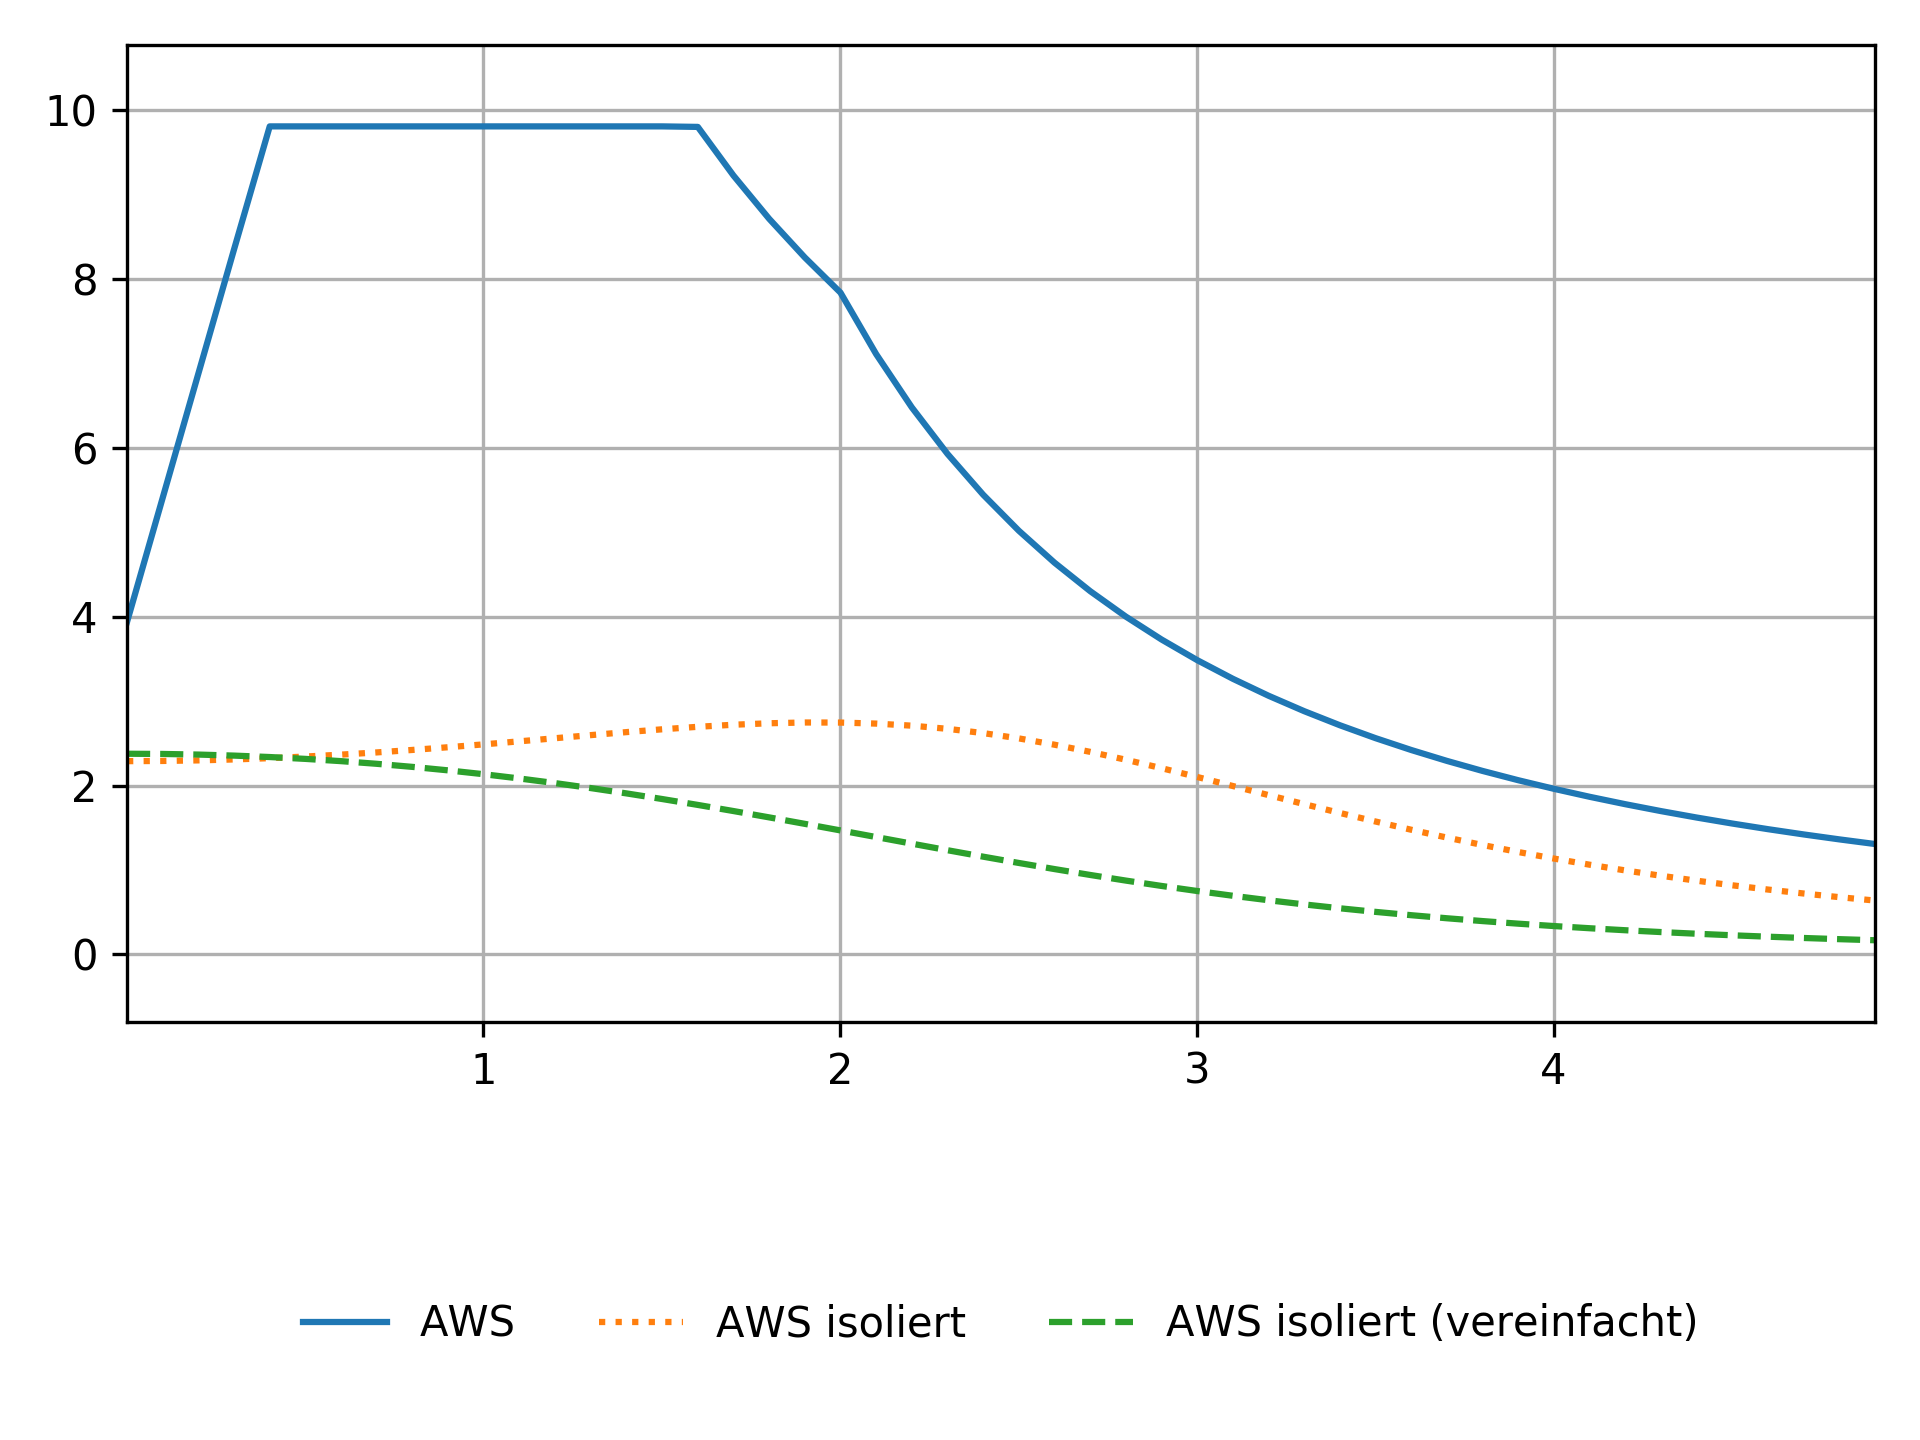
\includegraphics[width=1.0\textwidth]{Isolation.png}
    \caption{Isolationsspektren der drei Ansätze}
    \label{fig:Isolation}
\end{figure}

Wie zu erwarten war, ist die Modellierung als effektiver Einmassenschwinger nur eine Näherung. Die Ergebnisse über die Transmissibilität liefern durchweg etwas größere Beschleunigungen als der vereinfachte Ansatz, wobei diese Differenz in der Nähe der Isolatorperiode sich stärker ausprägt. Auch ist anzumerken, dass die Isolationsspektren geglättet sind, da sie aus dem ebenfalls bereits geglätteten Antwortspektrum berechnet wurden.

Um auch einen Vergleich mit den numerisch ermittelten Werten aus \cite{Isemann} zu machen wurde das Beispiel in Kapitel 11.3 untersucht.
Mit den angegebenen Massen und der Isolatorsteifigkeit stimmt jedoch die Periode des Isolators, die mit $T = 2.251 s$ angeben wurde nicht überein.

\begin{align*}
T &= \frac{2 np.pi}{\sqrt{(k_2/(m_2+m_1))}}\\
  &= \frac{2 np.pi}{\sqrt{(32000/( 2846.7 t + 1619.5 t)}}\\
  &= 2.347 s \neq 2.251 s
\end{align*}

Die Vermutung liegt nahe, dass für $m_1$ die Masse aus dem vorrangegangenen Beispiel in den Berechnungen verwendet wurde und es sich in den Angaben um einen \glqq Zahlendreher\grqq{} handelt.

\begin{align*}
T &= \frac{2 np.pi}{\sqrt{(32000/( 2486.7 t + 1619.5 t)}}\\
  &= 2.251 s = 2.251 s
\end{align*}

Mit dieser Vermutung bestätigt wird weiterhin mit $m_1 = 2486.7 t$ gerechnet.
Aus der angebenen Steifigkeit für den Isolator von $k_2 = 32000 kN/m$ lässt sich der verwendete Radius und das Dämpfungsmaß bestimmen.

\begin{align*}
k_2 &= \frac{G}{R} + \mu \frac{G}{D}\\
    &= \frac{41062 kN}{R} + 0.05 \cdot \frac{41062 kN}{0.325 m} = 32000 kN/m \Rightarrow R = 1.777 m
\end{align*}

\begin{equation*}
\xi_2 = \xi_{eff} = \frac{2}{\pi} \frac{\mu R}{(D + \mu R)} = \frac{2}{\pi} \frac{0.05 \cdot 1.777 m}{(0.325 m + 0.05 \cdot 1.777 m)} \approx 0.1367
\end{equation*} 

\makebox[1cm]{$D$}    = 0.325 m \par
\makebox[1cm]{$\mu$}  = 0.05\par
\makebox[1cm]{$m_1$}  = 2486.7 t\par
\makebox[1cm]{$m_2$}  = 1619.5 t\par
\makebox[1cm]{$k_2$}  = 32000 kN/m \par
\makebox[1cm]{$R$}    = 1.777 m\par

\begin{figure}[H]
    \centering
    \includegraphics[width=1.0\textwidth]{_Isolation_2.png}
    \caption{Vergleich der Isolationsspektren aus Zeitschrittberechnung \cite{Isemann}, vereinfachten Ansatz und Ansatz der Transmissibilität}
    \label{fig:Isolation}
\end{figure}

Hier wird deutlich, dass beide Ansätze auf der unsicheren Seite liegen. Bei dem Ansatz der Transmissibilität liegt die Vermutung nahe, dass durch die Bestimmung der Beschleunigung am gedämpften Antwortspektrum eine doppelte Berücksichtigung der Dämpfung zufolge hatte, da diese bereits in den Transmissibilitätkoeffizienten erfasst wurde.
Eine Anpassung (\cref{fig:Isolation2}) mit $\eta = 1.0$ zeigt, dass das Isolationsspektrum nun eine Einhüllende darstellt, allerdings auch deutlich auf der sicheren Seite liegt.

\begin{figure}[H]
    \centering
    \includegraphics[width=1.0\textwidth]{_Isolation_3.png}
    \caption{Vergleich der Isolationsspektren aus Zeitschrittberechnung \cite{Isemann}, vereinfachten Ansatz und Ansatz der Transmissibilität ($\eta = 1$)}
    \label{fig:Isolation2}
\end{figure}

\pagebreak